\documentclass[1p]{elsarticle_modified}
%\bibliographystyle{elsarticle-num}

%\usepackage[colorlinks]{hyperref}
%\usepackage{abbrmath_seonhwa} %\Abb, \Ascr, \Acal ,\Abf, \Afrak
\usepackage{amsfonts}
\usepackage{amssymb}
\usepackage{amsmath}
\usepackage{amsthm}
\usepackage{scalefnt}
\usepackage{amsbsy}
\usepackage{kotex}
\usepackage{caption}
\usepackage{subfig}
\usepackage{color}
\usepackage{graphicx}
\usepackage{xcolor} %% white, black, red, green, blue, cyan, magenta, yellow
\usepackage{float}
\usepackage{setspace}
\usepackage{hyperref}

\usepackage{tikz}
\usetikzlibrary{arrows}

\usepackage{multirow}
\usepackage{array} % fixed length table
\usepackage{hhline}

%%%%%%%%%%%%%%%%%%%%%
\makeatletter
\renewcommand*\env@matrix[1][\arraystretch]{%
	\edef\arraystretch{#1}%
	\hskip -\arraycolsep
	\let\@ifnextchar\new@ifnextchar
	\array{*\c@MaxMatrixCols c}}
\makeatother %https://tex.stackexchange.com/questions/14071/how-can-i-increase-the-line-spacing-in-a-matrix
%%%%%%%%%%%%%%%

\usepackage[normalem]{ulem}

\newcommand{\msout}[1]{\ifmmode\text{\sout{\ensuremath{#1}}}\else\sout{#1}\fi}
%SOURCE: \msout is \stkout macro in https://tex.stackexchange.com/questions/20609/strikeout-in-math-mode

\newcommand{\cancel}[1]{
	\ifmmode
	{\color{red}\msout{#1}}
	\else
	{\color{red}\sout{#1}}
	\fi
}

\newcommand{\add}[1]{
	{\color{blue}\uwave{#1}}
}

\newcommand{\replace}[2]{
	\ifmmode
	{\color{red}\msout{#1}}{\color{blue}\uwave{#2}}
	\else
	{\color{red}\sout{#1}}{\color{blue}\uwave{#2}}
	\fi
}

\newcommand{\Sol}{\mathcal{S}} %segment
\newcommand{\D}{D} %diagram
\newcommand{\A}{\mathcal{A}} %arc


%%%%%%%%%%%%%%%%%%%%%%%%%%%%%5 test

\def\sl{\operatorname{\textup{SL}}(2,\Cbb)}
\def\psl{\operatorname{\textup{PSL}}(2,\Cbb)}
\def\quan{\mkern 1mu \triangleright \mkern 1mu}

\theoremstyle{definition}
\newtheorem{thm}{Theorem}[section]
\newtheorem{prop}[thm]{Proposition}
\newtheorem{lem}[thm]{Lemma}
\newtheorem{ques}[thm]{Question}
\newtheorem{cor}[thm]{Corollary}
\newtheorem{defn}[thm]{Definition}
\newtheorem{exam}[thm]{Example}
\newtheorem{rmk}[thm]{Remark}
\newtheorem{alg}[thm]{Algorithm}

\newcommand{\I}{\sqrt{-1}}
\begin{document}

%\begin{frontmatter}
%
%\title{Boundary parabolic representations of knots up to 8 crossings}
%
%%% Group authors per affiliation:
%\author{Yunhi Cho} 
%\address{Department of Mathematics, University of Seoul, Seoul, Korea}
%\ead{yhcho@uos.ac.kr}
%
%
%\author{Seonhwa Kim} %\fnref{s_kim}}
%\address{Center for Geometry and Physics, Institute for Basic Science, Pohang, 37673, Korea}
%\ead{ryeona17@ibs.re.kr}
%
%\author{Hyuk Kim}
%\address{Department of Mathematical Sciences, Seoul National University, Seoul 08826, Korea}
%\ead{hyukkim@snu.ac.kr}
%
%\author{Seokbeom Yoon}
%\address{Department of Mathematical Sciences, Seoul National University, Seoul, 08826,  Korea}
%\ead{sbyoon15@snu.ac.kr}
%
%\begin{abstract}
%We find all boundary parabolic representation of knots up to 8 crossings.
%
%\end{abstract}
%\begin{keyword}
%    \MSC[2010] 57M25 
%\end{keyword}
%
%\end{frontmatter}

%\linenumbers
%\tableofcontents
%
\newcommand\colored[1]{\textcolor{white}{\rule[-0.35ex]{0.8em}{1.4ex}}\kern-0.8em\color{red} #1}%
%\newcommand\colored[1]{\textcolor{white}{ #1}\kern-2.17ex	\textcolor{white}{ #1}\kern-1.81ex	\textcolor{white}{ #1}\kern-2.15ex\color{red}#1	}

{\Large $\underline{12a_{0509}~(K12a_{0509})}$}

\setlength{\tabcolsep}{10pt}
\renewcommand{\arraystretch}{1.6}
\vspace{1cm}\begin{tabular}{m{100pt}>{\centering\arraybackslash}m{274pt}}
\multirow{5}{120pt}{
	\centering
	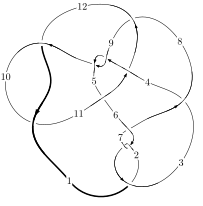
\includegraphics[width=112pt]{../../../GIT/diagram.site/Diagrams/png/1310_12a_0509.png}\\
\ \ \ A knot diagram\footnotemark}&
\allowdisplaybreaks
\textbf{Linearized knot diagam} \\
\cline{2-2}
 &
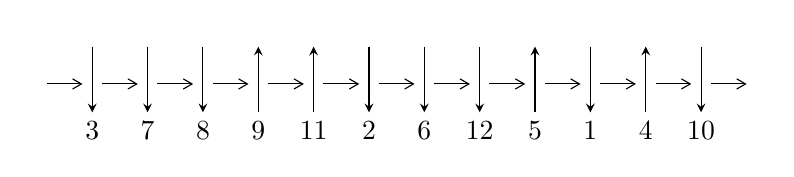
\begin{tikzpicture}[x=20pt, y=17pt]
	% nodes
	\node (C0) at (0, 0) {};
	\node (C1) at (1, 0) {};
	\node (C1U) at (1, +1) {};
	\node (C1D) at (1, -1) {3};

	\node (C2) at (2, 0) {};
	\node (C2U) at (2, +1) {};
	\node (C2D) at (2, -1) {7};

	\node (C3) at (3, 0) {};
	\node (C3U) at (3, +1) {};
	\node (C3D) at (3, -1) {8};

	\node (C4) at (4, 0) {};
	\node (C4U) at (4, +1) {};
	\node (C4D) at (4, -1) {9};

	\node (C5) at (5, 0) {};
	\node (C5U) at (5, +1) {};
	\node (C5D) at (5, -1) {11};

	\node (C6) at (6, 0) {};
	\node (C6U) at (6, +1) {};
	\node (C6D) at (6, -1) {2};

	\node (C7) at (7, 0) {};
	\node (C7U) at (7, +1) {};
	\node (C7D) at (7, -1) {6};

	\node (C8) at (8, 0) {};
	\node (C8U) at (8, +1) {};
	\node (C8D) at (8, -1) {12};

	\node (C9) at (9, 0) {};
	\node (C9U) at (9, +1) {};
	\node (C9D) at (9, -1) {5};

	\node (C10) at (10, 0) {};
	\node (C10U) at (10, +1) {};
	\node (C10D) at (10, -1) {1};

	\node (C11) at (11, 0) {};
	\node (C11U) at (11, +1) {};
	\node (C11D) at (11, -1) {4};

	\node (C12) at (12, 0) {};
	\node (C12U) at (12, +1) {};
	\node (C12D) at (12, -1) {10};
	\node (C13) at (13, 0) {};

	% arrows
	\draw[->,>={angle 60}]
	(C0) edge (C1) (C1) edge (C2) (C2) edge (C3) (C3) edge (C4) (C4) edge (C5) (C5) edge (C6) (C6) edge (C7) (C7) edge (C8) (C8) edge (C9) (C9) edge (C10) (C10) edge (C11) (C11) edge (C12) (C12) edge (C13) ;	\draw[->,>=stealth]
	(C1U) edge (C1D) (C2U) edge (C2D) (C3U) edge (C3D) (C4D) edge (C4U) (C5D) edge (C5U) (C6U) edge (C6D) (C7U) edge (C7D) (C8U) edge (C8D) (C9D) edge (C9U) (C10U) edge (C10D) (C11D) edge (C11U) (C12U) edge (C12D) ;
	\end{tikzpicture} \\
\hhline{~~} \\& 
\textbf{Solving Sequence} \\ \cline{2-2} 
 &
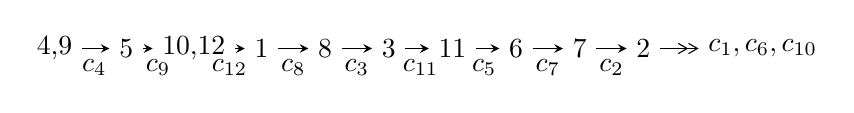
\begin{tikzpicture}[x=23pt, y=7pt]
	% node
	\node (A0) at (-1/8, 0) {4,9};
	\node (A1) at (1, 0) {5};
	\node (A2) at (33/16, 0) {10,12};
	\node (A3) at (25/8, 0) {1};
	\node (A4) at (33/8, 0) {8};
	\node (A5) at (41/8, 0) {3};
	\node (A6) at (49/8, 0) {11};
	\node (A7) at (57/8, 0) {6};
	\node (A8) at (65/8, 0) {7};
	\node (A9) at (73/8, 0) {2};
	\node (C1) at (1/2, -1) {$c_{4}$};
	\node (C2) at (3/2, -1) {$c_{9}$};
	\node (C3) at (21/8, -1) {$c_{12}$};
	\node (C4) at (29/8, -1) {$c_{8}$};
	\node (C5) at (37/8, -1) {$c_{3}$};
	\node (C6) at (45/8, -1) {$c_{11}$};
	\node (C7) at (53/8, -1) {$c_{5}$};
	\node (C8) at (61/8, -1) {$c_{7}$};
	\node (C9) at (69/8, -1) {$c_{2}$};
	\node (A10) at (11, 0) {$c_{1},c_{6},c_{10}$};

	% edge
	\draw[->,>=stealth]	
	(A0) edge (A1) (A1) edge (A2) (A2) edge (A3) (A3) edge (A4) (A4) edge (A5) (A5) edge (A6) (A6) edge (A7) (A7) edge (A8) (A8) edge (A9) ;
	\draw[->>,>={angle 60}]	
	(A9) edge (A10);
\end{tikzpicture} \\ 

\end{tabular} \\

\footnotetext{
The image of knot diagram is generated by the software ``\textbf{Draw programme}" developed by Andrew Bartholomew(\url{http://www.layer8.co.uk/maths/draw/index.htm\#Running-draw}), where we modified some parts for our purpose(\url{https://github.com/CATsTAILs/LinksPainter}).
}\phantom \\ \newline 
\centering \textbf{Ideals for irreducible components\footnotemark of $X_{\text{par}}$} 
 
\begin{align*}
I^u_{1}&=\langle 
-1.78105\times10^{290} u^{107}+1.60836\times10^{290} u^{106}+\cdots+3.54086\times10^{291} b-2.25324\times10^{291},\\
\phantom{I^u_{1}}&\phantom{= \langle  }-1.68797\times10^{292} u^{107}+7.50224\times10^{291} u^{106}+\cdots+1.16848\times10^{293} a-1.63357\times10^{293},\\
\phantom{I^u_{1}}&\phantom{= \langle  }u^{108}-2 u^{107}+\cdots-3 u^2+1\rangle \\
I^u_{2}&=\langle 
b,\;a+1,\;u+1\rangle \\
\\
\end{align*}
\raggedright * 2 irreducible components of $\dim_{\mathbb{C}}=0$, with total 109 representations.\\
\footnotetext{All coefficients of polynomials are rational numbers. But the coefficients are sometimes approximated in decimal forms when there is not enough margin.}
\newpage
\renewcommand{\arraystretch}{1}
\centering \section*{I. $I^u_{1}= \langle -1.78\times10^{290} u^{107}+1.61\times10^{290} u^{106}+\cdots+3.54\times10^{291} b-2.25\times10^{291},\;-1.69\times10^{292} u^{107}+7.50\times10^{291} u^{106}+\cdots+1.17\times10^{293} a-1.63\times10^{293},\;u^{108}-2 u^{107}+\cdots-3 u^2+1 \rangle$}
\flushleft \textbf{(i) Arc colorings}\\
\begin{tabular}{m{7pt} m{180pt} m{7pt} m{180pt} }
\flushright $a_{4}=$&$\begin{pmatrix}1\\0\end{pmatrix}$ \\
\flushright $a_{9}=$&$\begin{pmatrix}0\\u\end{pmatrix}$ \\
\flushright $a_{5}=$&$\begin{pmatrix}1\\- u^2\end{pmatrix}$ \\
\flushright $a_{10}=$&$\begin{pmatrix}u\\- u^3+u\end{pmatrix}$ \\
\flushright $a_{12}=$&$\begin{pmatrix}0.144459 u^{107}-0.0642050 u^{106}+\cdots-0.623690 u+1.39803\\0.0503000 u^{107}-0.0454230 u^{106}+\cdots+1.89807 u+0.636356\end{pmatrix}$ \\
\flushright $a_{1}=$&$\begin{pmatrix}0.0112300 u^{107}+0.207726 u^{106}+\cdots-1.38853 u+0.756202\\- u^3+u\end{pmatrix}$ \\
\flushright $a_{8}=$&$\begin{pmatrix}3.64516 u^{107}-3.71116 u^{106}+\cdots-2.65234 u-6.17436\\-0.146240 u^{107}+0.203332 u^{106}+\cdots-0.752096 u-1.29717\end{pmatrix}$ \\
\flushright $a_{3}=$&$\begin{pmatrix}2.16323 u^{107}-2.00756 u^{106}+\cdots-1.52409 u-0.229475\\0.0623410 u^{107}+0.0227712 u^{106}+\cdots+0.941552 u+0.128731\end{pmatrix}$ \\
\flushright $a_{11}=$&$\begin{pmatrix}0.0941586 u^{107}-0.0187819 u^{106}+\cdots-2.52176 u+0.761675\\0.0503000 u^{107}-0.0454230 u^{106}+\cdots+1.89807 u+0.636356\end{pmatrix}$ \\
\flushright $a_{6}=$&$\begin{pmatrix}-4.66146 u^{107}+5.27089 u^{106}+\cdots+2.68247 u+6.80830\\-0.304016 u^{107}+0.592629 u^{106}+\cdots-0.844491 u-0.264806\end{pmatrix}$ \\
\flushright $a_{7}=$&$\begin{pmatrix}3.63714 u^{107}-3.05931 u^{106}+\cdots+0.937464 u-4.97673\\-0.184958 u^{107}+0.337994 u^{106}+\cdots-1.11297 u-0.562464\end{pmatrix}$ \\
\flushright $a_{2}=$&$\begin{pmatrix}1.98561 u^{107}-1.42635 u^{106}+\cdots-5.91663 u-1.39635\\-0.121188 u^{107}+0.380071 u^{106}+\cdots+0.892331 u-0.0283241\end{pmatrix}$\\&\end{tabular}
\flushleft \textbf{(ii) Obstruction class $= -1$}\\~\\
\flushleft \textbf{(iii) Cusp Shapes $= 3.32154 u^{107}-2.84726 u^{106}+\cdots-14.1969 u-3.91869$}\\~\\
\newpage\renewcommand{\arraystretch}{1}
\flushleft \textbf{(iv) u-Polynomials at the component}\newline \\
\begin{tabular}{m{50pt}|m{274pt}}
Crossings & \hspace{64pt}u-Polynomials at each crossing \\
\hline $$\begin{aligned}c_{1},c_{7}\end{aligned}$$&$\begin{aligned}
&u^{108}+36 u^{107}+\cdots+6 u+1
\end{aligned}$\\
\hline $$\begin{aligned}c_{2},c_{6}\end{aligned}$$&$\begin{aligned}
&u^{108}-2 u^{107}+\cdots-2 u+1
\end{aligned}$\\
\hline $$\begin{aligned}c_{3}\end{aligned}$$&$\begin{aligned}
&u^{108}+4 u^{107}+\cdots+487368 u+75901
\end{aligned}$\\
\hline $$\begin{aligned}c_{4},c_{9}\end{aligned}$$&$\begin{aligned}
&u^{108}-2 u^{107}+\cdots-3 u^2+1
\end{aligned}$\\
\hline $$\begin{aligned}c_{5}\end{aligned}$$&$\begin{aligned}
&33(33 u^{108}+126 u^{107}+\cdots+888 u-139)
\end{aligned}$\\
\hline $$\begin{aligned}c_{8}\end{aligned}$$&$\begin{aligned}
&33(33 u^{108}-390 u^{107}+\cdots+18 u-1)
\end{aligned}$\\
\hline $$\begin{aligned}c_{10},c_{12}\end{aligned}$$&$\begin{aligned}
&u^{108}-3 u^{107}+\cdots-618 u+49
\end{aligned}$\\
\hline $$\begin{aligned}c_{11}\end{aligned}$$&$\begin{aligned}
&u^{108}-3 u^{107}+\cdots-384 u-231
\end{aligned}$\\
\hline
\end{tabular}\\~\\
\newpage\renewcommand{\arraystretch}{1}
\flushleft \textbf{(v) Riley Polynomials at the component}\newline \\
\begin{tabular}{m{50pt}|m{274pt}}
Crossings & \hspace{64pt}Riley Polynomials at each crossing \\
\hline $$\begin{aligned}c_{1},c_{7}\end{aligned}$$&$\begin{aligned}
&y^{108}+72 y^{107}+\cdots+18 y+1
\end{aligned}$\\
\hline $$\begin{aligned}c_{2},c_{6}\end{aligned}$$&$\begin{aligned}
&y^{108}-36 y^{107}+\cdots-6 y+1
\end{aligned}$\\
\hline $$\begin{aligned}c_{3}\end{aligned}$$&$\begin{aligned}
&y^{108}-48 y^{107}+\cdots-182916038914 y+5760961801
\end{aligned}$\\
\hline $$\begin{aligned}c_{4},c_{9}\end{aligned}$$&$\begin{aligned}
&y^{108}-64 y^{107}+\cdots-6 y+1
\end{aligned}$\\
\hline $$\begin{aligned}c_{5}\end{aligned}$$&$\begin{aligned}
&1089(1089 y^{108}+76788 y^{107}+\cdots-1572226 y+19321)
\end{aligned}$\\
\hline $$\begin{aligned}c_{8}\end{aligned}$$&$\begin{aligned}
&1089(1089 y^{108}+74412 y^{107}+\cdots-206 y+1)
\end{aligned}$\\
\hline $$\begin{aligned}c_{10},c_{12}\end{aligned}$$&$\begin{aligned}
&y^{108}-69 y^{107}+\cdots-277554 y+2401
\end{aligned}$\\
\hline $$\begin{aligned}c_{11}\end{aligned}$$&$\begin{aligned}
&y^{108}-9 y^{107}+\cdots+893430 y+53361
\end{aligned}$\\
\hline
\end{tabular}\\~\\
\newpage\flushleft \textbf{(vi) Complex Volumes and Cusp Shapes}
$$\begin{array}{c|c|c}  
\text{Solutions to }I^u_{1}& \I (\text{vol} + \sqrt{-1}CS) & \text{Cusp shape}\\
 \hline 
\begin{aligned}
u &= -0.925744 + 0.378027 I \\
a &= -0.424665 - 0.306104 I \\
b &= -0.69136 - 1.65988 I\end{aligned}
 & -0.33884 - 4.17825 I & \phantom{-0.000000 } 0 \\ \hline\begin{aligned}
u &= -0.925744 - 0.378027 I \\
a &= -0.424665 + 0.306104 I \\
b &= -0.69136 + 1.65988 I\end{aligned}
 & -0.33884 + 4.17825 I & \phantom{-0.000000 } 0 \\ \hline\begin{aligned}
u &= \phantom{-}0.921133 + 0.391082 I \\
a &= \phantom{-}0.466764 - 0.239826 I \\
b &= \phantom{-}0.76927 - 1.74937 I\end{aligned}
 & -1.46043 + 9.58568 I & \phantom{-0.000000 } 0 \\ \hline\begin{aligned}
u &= \phantom{-}0.921133 - 0.391082 I \\
a &= \phantom{-}0.466764 + 0.239826 I \\
b &= \phantom{-}0.76927 + 1.74937 I\end{aligned}
 & -1.46043 - 9.58568 I & \phantom{-0.000000 } 0 \\ \hline\begin{aligned}
u &= -0.848255 + 0.559300 I \\
a &= -0.789114 + 0.479083 I \\
b &= -0.645673 - 0.058019 I\end{aligned}
 & \phantom{-}2.99631 + 4.71722 I & \phantom{-0.000000 } 0 \\ \hline\begin{aligned}
u &= -0.848255 - 0.559300 I \\
a &= -0.789114 - 0.479083 I \\
b &= -0.645673 + 0.058019 I\end{aligned}
 & \phantom{-}2.99631 - 4.71722 I & \phantom{-0.000000 } 0 \\ \hline\begin{aligned}
u &= \phantom{-}1.014520 + 0.076956 I \\
a &= \phantom{-}2.45207 - 5.72196 I \\
b &= -0.021423 - 0.312109 I\end{aligned}
 & \phantom{-}1.77087 - 0.01042 I & \phantom{-0.000000 } 0 \\ \hline\begin{aligned}
u &= \phantom{-}1.014520 - 0.076956 I \\
a &= \phantom{-}2.45207 + 5.72196 I \\
b &= -0.021423 + 0.312109 I\end{aligned}
 & \phantom{-}1.77087 + 0.01042 I & \phantom{-0.000000 } 0 \\ \hline\begin{aligned}
u &= -1.026590 + 0.059563 I \\
a &= -4.51531 - 6.54930 I \\
b &= \phantom{-}0.084458 - 0.254370 I\end{aligned}
 & \phantom{-}0.89202 + 5.38333 I & \phantom{-0.000000 } 0 \\ \hline\begin{aligned}
u &= -1.026590 - 0.059563 I \\
a &= -4.51531 + 6.54930 I \\
b &= \phantom{-}0.084458 + 0.254370 I\end{aligned}
 & \phantom{-}0.89202 - 5.38333 I & \phantom{-0.000000 } 0\\
 \hline 
 \end{array}$$\newpage$$\begin{array}{c|c|c}  
\text{Solutions to }I^u_{1}& \I (\text{vol} + \sqrt{-1}CS) & \text{Cusp shape}\\
 \hline 
\begin{aligned}
u &= \phantom{-}0.890427 + 0.380807 I \\
a &= \phantom{-}0.303584 - 0.136076 I \\
b &= \phantom{-}0.96363 - 1.55607 I\end{aligned}
 & -5.87089 + 3.60473 I & \phantom{-0.000000 } 0 \\ \hline\begin{aligned}
u &= \phantom{-}0.890427 - 0.380807 I \\
a &= \phantom{-}0.303584 + 0.136076 I \\
b &= \phantom{-}0.96363 + 1.55607 I\end{aligned}
 & -5.87089 - 3.60473 I & \phantom{-0.000000 } 0 \\ \hline\begin{aligned}
u &= -0.402522 + 0.872226 I \\
a &= -0.851587 + 0.024864 I \\
b &= -0.769645 - 0.059732 I\end{aligned}
 & \phantom{-}3.17014 + 4.56924 I & \phantom{-0.000000 } 0 \\ \hline\begin{aligned}
u &= -0.402522 - 0.872226 I \\
a &= -0.851587 - 0.024864 I \\
b &= -0.769645 + 0.059732 I\end{aligned}
 & \phantom{-}3.17014 - 4.56924 I & \phantom{-0.000000 } 0 \\ \hline\begin{aligned}
u &= \phantom{-}1.038340 + 0.189468 I \\
a &= \phantom{-}1.17845 - 1.13861 I \\
b &= -0.015139 - 0.648279 I\end{aligned}
 & \phantom{-}2.69941 + 0.12491 I & \phantom{-0.000000 } 0 \\ \hline\begin{aligned}
u &= \phantom{-}1.038340 - 0.189468 I \\
a &= \phantom{-}1.17845 + 1.13861 I \\
b &= -0.015139 + 0.648279 I\end{aligned}
 & \phantom{-}2.69941 - 0.12491 I & \phantom{-0.000000 } 0 \\ \hline\begin{aligned}
u &= \phantom{-}0.927128 + 0.143943 I \\
a &= -0.74188 - 2.07907 I \\
b &= \phantom{-}0.334650 - 0.476961 I\end{aligned}
 & -0.117691 + 0.649963 I & \phantom{-0.000000 } 0 \\ \hline\begin{aligned}
u &= \phantom{-}0.927128 - 0.143943 I \\
a &= -0.74188 + 2.07907 I \\
b &= \phantom{-}0.334650 + 0.476961 I\end{aligned}
 & -0.117691 - 0.649963 I & \phantom{-0.000000 } 0 \\ \hline\begin{aligned}
u &= -0.888497 + 0.299241 I \\
a &= \phantom{-}0.062931 - 0.490294 I \\
b &= -0.714295 - 1.060540 I\end{aligned}
 & -1.24184 - 2.64418 I & \phantom{-0.000000 } 0 \\ \hline\begin{aligned}
u &= -0.888497 - 0.299241 I \\
a &= \phantom{-}0.062931 + 0.490294 I \\
b &= -0.714295 + 1.060540 I\end{aligned}
 & -1.24184 + 2.64418 I & \phantom{-0.000000 } 0\\
 \hline 
 \end{array}$$\newpage$$\begin{array}{c|c|c}  
\text{Solutions to }I^u_{1}& \I (\text{vol} + \sqrt{-1}CS) & \text{Cusp shape}\\
 \hline 
\begin{aligned}
u &= -1.052240 + 0.179848 I \\
a &= -1.26879 - 0.62622 I \\
b &= \phantom{-}0.041151 - 0.545307 I\end{aligned}
 & \phantom{-}2.10034 - 5.29369 I & \phantom{-0.000000 } 0 \\ \hline\begin{aligned}
u &= -1.052240 - 0.179848 I \\
a &= -1.26879 + 0.62622 I \\
b &= \phantom{-}0.041151 + 0.545307 I\end{aligned}
 & \phantom{-}2.10034 + 5.29369 I & \phantom{-0.000000 } 0 \\ \hline\begin{aligned}
u &= \phantom{-}0.848712 + 0.369880 I \\
a &= \phantom{-}0.0752943 + 0.0150683 I \\
b &= \phantom{-}1.17863 - 1.30099 I\end{aligned}
 & -2.21585 - 2.34815 I & \phantom{-0.000000 } 0 \\ \hline\begin{aligned}
u &= \phantom{-}0.848712 - 0.369880 I \\
a &= \phantom{-}0.0752943 - 0.0150683 I \\
b &= \phantom{-}1.17863 + 1.30099 I\end{aligned}
 & -2.21585 + 2.34815 I & \phantom{-0.000000 } 0 \\ \hline\begin{aligned}
u &= -0.848985 + 0.329851 I \\
a &= \phantom{-}0.111920 - 0.165045 I \\
b &= -1.00757 - 1.09207 I\end{aligned}
 & -1.16913 - 2.62387 I & \phantom{-0.000000 } 0 \\ \hline\begin{aligned}
u &= -0.848985 - 0.329851 I \\
a &= \phantom{-}0.111920 + 0.165045 I \\
b &= -1.00757 + 1.09207 I\end{aligned}
 & -1.16913 + 2.62387 I & \phantom{-0.000000 } 0 \\ \hline\begin{aligned}
u &= -1.061310 + 0.305657 I \\
a &= -0.598212 - 0.788151 I \\
b &= \phantom{-}0.305065 - 1.165900 I\end{aligned}
 & \phantom{-}2.24352 - 4.94196 I & \phantom{-0.000000 } 0 \\ \hline\begin{aligned}
u &= -1.061310 - 0.305657 I \\
a &= -0.598212 + 0.788151 I \\
b &= \phantom{-}0.305065 + 1.165900 I\end{aligned}
 & \phantom{-}2.24352 + 4.94196 I & \phantom{-0.000000 } 0 \\ \hline\begin{aligned}
u &= \phantom{-}0.120929 + 1.104430 I \\
a &= \phantom{-}0.732120 - 0.854405 I \\
b &= \phantom{-}0.871944 - 0.960259 I\end{aligned}
 & -3.64394 - 12.82890 I & \phantom{-0.000000 } 0 \\ \hline\begin{aligned}
u &= \phantom{-}0.120929 - 1.104430 I \\
a &= \phantom{-}0.732120 + 0.854405 I \\
b &= \phantom{-}0.871944 + 0.960259 I\end{aligned}
 & -3.64394 + 12.82890 I & \phantom{-0.000000 } 0\\
 \hline 
 \end{array}$$\newpage$$\begin{array}{c|c|c}  
\text{Solutions to }I^u_{1}& \I (\text{vol} + \sqrt{-1}CS) & \text{Cusp shape}\\
 \hline 
\begin{aligned}
u &= -0.132220 + 1.107000 I \\
a &= -0.723155 - 0.803219 I \\
b &= -0.850918 - 0.901810 I\end{aligned}
 & -2.37530 + 7.05611 I & \phantom{-0.000000 } 0 \\ \hline\begin{aligned}
u &= -0.132220 - 1.107000 I \\
a &= -0.723155 + 0.803219 I \\
b &= -0.850918 + 0.901810 I\end{aligned}
 & -2.37530 - 7.05611 I & \phantom{-0.000000 } 0 \\ \hline\begin{aligned}
u &= \phantom{-}0.118718 + 1.137740 I \\
a &= \phantom{-}0.584529 - 0.837104 I \\
b &= \phantom{-}0.694229 - 0.966561 I\end{aligned}
 & -8.92521 - 6.29536 I & \phantom{-0.000000 } 0 \\ \hline\begin{aligned}
u &= \phantom{-}0.118718 - 1.137740 I \\
a &= \phantom{-}0.584529 + 0.837104 I \\
b &= \phantom{-}0.694229 + 0.966561 I\end{aligned}
 & -8.92521 + 6.29536 I & \phantom{-0.000000 } 0 \\ \hline\begin{aligned}
u &= \phantom{-}0.920607 + 0.684791 I \\
a &= \phantom{-}0.604950 + 0.505920 I \\
b &= \phantom{-}0.677981 + 0.023970 I\end{aligned}
 & \phantom{-}3.79025 + 1.05337 I & \phantom{-0.000000 } 0 \\ \hline\begin{aligned}
u &= \phantom{-}0.920607 - 0.684791 I \\
a &= \phantom{-}0.604950 - 0.505920 I \\
b &= \phantom{-}0.677981 - 0.023970 I\end{aligned}
 & \phantom{-}3.79025 - 1.05337 I & \phantom{-0.000000 } 0 \\ \hline\begin{aligned}
u &= -0.157182 + 1.163090 I \\
a &= -0.539188 - 0.679767 I \\
b &= -0.618550 - 0.791581 I\end{aligned}
 & -4.09827 + 3.93224 I & \phantom{-0.000000 } 0 \\ \hline\begin{aligned}
u &= -0.157182 - 1.163090 I \\
a &= -0.539188 + 0.679767 I \\
b &= -0.618550 + 0.791581 I\end{aligned}
 & -4.09827 - 3.93224 I & \phantom{-0.000000 } 0 \\ \hline\begin{aligned}
u &= \phantom{-}1.124520 + 0.348742 I \\
a &= \phantom{-}0.578466 - 0.825190 I \\
b &= -0.83558 - 1.22876 I\end{aligned}
 & \phantom{-}1.94202 + 0.30856 I & \phantom{-0.000000 } 0 \\ \hline\begin{aligned}
u &= \phantom{-}1.124520 - 0.348742 I \\
a &= \phantom{-}0.578466 + 0.825190 I \\
b &= -0.83558 + 1.22876 I\end{aligned}
 & \phantom{-}1.94202 - 0.30856 I & \phantom{-0.000000 } 0\\
 \hline 
 \end{array}$$\newpage$$\begin{array}{c|c|c}  
\text{Solutions to }I^u_{1}& \I (\text{vol} + \sqrt{-1}CS) & \text{Cusp shape}\\
 \hline 
\begin{aligned}
u &= \phantom{-}0.359054 + 0.726041 I \\
a &= \phantom{-}0.950975 + 0.191225 I \\
b &= \phantom{-}0.759127 + 0.105143 I\end{aligned}
 & \phantom{-}3.58114 + 1.18791 I & \phantom{-}1.84333 + 0. I\phantom{ +0.000000I} \\ \hline\begin{aligned}
u &= \phantom{-}0.359054 - 0.726041 I \\
a &= \phantom{-}0.950975 - 0.191225 I \\
b &= \phantom{-}0.759127 - 0.105143 I\end{aligned}
 & \phantom{-}3.58114 - 1.18791 I & \phantom{-}1.84333 + 0. I\phantom{ +0.000000I} \\ \hline\begin{aligned}
u &= \phantom{-}0.119524 + 1.202100 I \\
a &= \phantom{-}0.382622 - 0.727957 I \\
b &= \phantom{-}0.445296 - 0.864404 I\end{aligned}
 & -6.28289 + 0.74941 I & \phantom{-0.000000 } 0 \\ \hline\begin{aligned}
u &= \phantom{-}0.119524 - 1.202100 I \\
a &= \phantom{-}0.382622 + 0.727957 I \\
b &= \phantom{-}0.445296 + 0.864404 I\end{aligned}
 & -6.28289 - 0.74941 I & \phantom{-0.000000 } 0 \\ \hline\begin{aligned}
u &= \phantom{-}1.161530 + 0.383511 I \\
a &= \phantom{-}0.517820 - 0.931592 I \\
b &= -1.26404 - 1.22400 I\end{aligned}
 & -0.91867 + 6.16427 I & \phantom{-0.000000 } 0 \\ \hline\begin{aligned}
u &= \phantom{-}1.161530 - 0.383511 I \\
a &= \phantom{-}0.517820 + 0.931592 I \\
b &= -1.26404 + 1.22400 I\end{aligned}
 & -0.91867 - 6.16427 I & \phantom{-0.000000 } 0 \\ \hline\begin{aligned}
u &= \phantom{-}1.210810 + 0.192388 I \\
a &= \phantom{-}0.512975 - 0.445035 I \\
b &= -0.620722 - 0.356967 I\end{aligned}
 & \phantom{-}2.76716 + 0.74119 I & \phantom{-0.000000 } 0 \\ \hline\begin{aligned}
u &= \phantom{-}1.210810 - 0.192388 I \\
a &= \phantom{-}0.512975 + 0.445035 I \\
b &= -0.620722 + 0.356967 I\end{aligned}
 & \phantom{-}2.76716 - 0.74119 I & \phantom{-0.000000 } 0 \\ \hline\begin{aligned}
u &= -1.179740 + 0.354059 I \\
a &= -0.456047 - 0.852388 I \\
b &= \phantom{-}1.15794 - 0.95235 I\end{aligned}
 & \phantom{-}3.30225 - 4.39680 I & \phantom{-0.000000 } 0 \\ \hline\begin{aligned}
u &= -1.179740 - 0.354059 I \\
a &= -0.456047 + 0.852388 I \\
b &= \phantom{-}1.15794 + 0.95235 I\end{aligned}
 & \phantom{-}3.30225 + 4.39680 I & \phantom{-0.000000 } 0\\
 \hline 
 \end{array}$$\newpage$$\begin{array}{c|c|c}  
\text{Solutions to }I^u_{1}& \I (\text{vol} + \sqrt{-1}CS) & \text{Cusp shape}\\
 \hline 
\begin{aligned}
u &= \phantom{-}1.179270 + 0.399117 I \\
a &= \phantom{-}0.469183 - 0.996289 I \\
b &= -1.48757 - 1.17355 I\end{aligned}
 & \phantom{-}4.03392 + 12.09010 I & \phantom{-0.000000 } 0 \\ \hline\begin{aligned}
u &= \phantom{-}1.179270 - 0.399117 I \\
a &= \phantom{-}0.469183 + 0.996289 I \\
b &= -1.48757 + 1.17355 I\end{aligned}
 & \phantom{-}4.03392 - 12.09010 I & \phantom{-0.000000 } 0 \\ \hline\begin{aligned}
u &= -1.184000 + 0.392776 I \\
a &= -0.448656 - 0.975463 I \\
b &= \phantom{-}1.45864 - 1.10051 I\end{aligned}
 & \phantom{-}5.12288 - 6.47021 I & \phantom{-0.000000 } 0 \\ \hline\begin{aligned}
u &= -1.184000 - 0.392776 I \\
a &= -0.448656 + 0.975463 I \\
b &= \phantom{-}1.45864 + 1.10051 I\end{aligned}
 & \phantom{-}5.12288 + 6.47021 I & \phantom{-0.000000 } 0 \\ \hline\begin{aligned}
u &= -1.251960 + 0.353472 I \\
a &= -0.235813 - 0.800576 I \\
b &= \phantom{-}1.34319 - 0.46896 I\end{aligned}
 & \phantom{-}8.08609 - 4.85702 I & \phantom{-0.000000 } 0 \\ \hline\begin{aligned}
u &= -1.251960 - 0.353472 I \\
a &= -0.235813 + 0.800576 I \\
b &= \phantom{-}1.34319 + 0.46896 I\end{aligned}
 & \phantom{-}8.08609 + 4.85702 I & \phantom{-0.000000 } 0 \\ \hline\begin{aligned}
u &= \phantom{-}1.266890 + 0.344460 I \\
a &= \phantom{-}0.203311 - 0.751783 I \\
b &= -1.293520 - 0.367706 I\end{aligned}
 & \phantom{-}7.96559 - 0.80034 I & \phantom{-0.000000 } 0 \\ \hline\begin{aligned}
u &= \phantom{-}1.266890 - 0.344460 I \\
a &= \phantom{-}0.203311 + 0.751783 I \\
b &= -1.293520 + 0.367706 I\end{aligned}
 & \phantom{-}7.96559 + 0.80034 I & \phantom{-0.000000 } 0 \\ \hline\begin{aligned}
u &= \phantom{-}0.571599 + 0.353726 I \\
a &= -1.18919 + 1.04297 I \\
b &= \phantom{-}1.54397 + 0.18503 I\end{aligned}
 & -2.93513 + 5.72866 I & -8.97675 - 7.05459 I \\ \hline\begin{aligned}
u &= \phantom{-}0.571599 - 0.353726 I \\
a &= -1.18919 - 1.04297 I \\
b &= \phantom{-}1.54397 - 0.18503 I\end{aligned}
 & -2.93513 - 5.72866 I & -8.97675 + 7.05459 I\\
 \hline 
 \end{array}$$\newpage$$\begin{array}{c|c|c}  
\text{Solutions to }I^u_{1}& \I (\text{vol} + \sqrt{-1}CS) & \text{Cusp shape}\\
 \hline 
\begin{aligned}
u &= -0.580654 + 0.313057 I \\
a &= \phantom{-}1.27402 + 0.86525 I \\
b &= -1.394500 + 0.092527 I\end{aligned}
 & -1.85726 - 0.55088 I & -6.98907 + 1.92903 I \\ \hline\begin{aligned}
u &= -0.580654 - 0.313057 I \\
a &= \phantom{-}1.27402 - 0.86525 I \\
b &= -1.394500 - 0.092527 I\end{aligned}
 & -1.85726 + 0.55088 I & -6.98907 - 1.92903 I \\ \hline\begin{aligned}
u &= -0.639538\phantom{ +0.000000I} \\
a &= -0.867624\phantom{ +0.000000I} \\
b &= -0.334991\phantom{ +0.000000I}\end{aligned}
 & -1.72228\phantom{ +0.000000I} & -4.61080\phantom{ +0.000000I} \\ \hline\begin{aligned}
u &= \phantom{-}0.001334 + 0.616486 I \\
a &= -1.50766 + 0.86763 I \\
b &= -0.713042 + 0.973471 I\end{aligned}
 & \phantom{-}0.67445 - 8.26204 I & -4.89690 + 7.40535 I \\ \hline\begin{aligned}
u &= \phantom{-}0.001334 - 0.616486 I \\
a &= -1.50766 - 0.86763 I \\
b &= -0.713042 - 0.973471 I\end{aligned}
 & \phantom{-}0.67445 + 8.26204 I & -4.89690 - 7.40535 I \\ \hline\begin{aligned}
u &= \phantom{-}0.500276 + 0.359081 I \\
a &= -1.43423 + 1.24440 I \\
b &= \phantom{-}1.40023 + 0.46950 I\end{aligned}
 & -6.87828 - 0.19248 I & -13.90816 - 1.39132 I \\ \hline\begin{aligned}
u &= \phantom{-}0.500276 - 0.359081 I \\
a &= -1.43423 - 1.24440 I \\
b &= \phantom{-}1.40023 - 0.46950 I\end{aligned}
 & -6.87828 + 0.19248 I & -13.90816 + 1.39132 I \\ \hline\begin{aligned}
u &= \phantom{-}1.240460 + 0.614749 I \\
a &= \phantom{-}0.003425 + 1.039780 I \\
b &= \phantom{-}1.081660 + 0.532522 I\end{aligned}
 & \phantom{-}6.13608 + 4.49586 I & \phantom{-0.000000 } 0 \\ \hline\begin{aligned}
u &= \phantom{-}1.240460 - 0.614749 I \\
a &= \phantom{-}0.003425 - 1.039780 I \\
b &= \phantom{-}1.081660 - 0.532522 I\end{aligned}
 & \phantom{-}6.13608 - 4.49586 I & \phantom{-0.000000 } 0 \\ \hline\begin{aligned}
u &= \phantom{-}0.021502 + 0.608380 I \\
a &= \phantom{-}1.42889 + 0.82516 I \\
b &= \phantom{-}0.701016 + 0.881446 I\end{aligned}
 & \phantom{-}1.69122 + 2.69833 I & -2.72518 - 2.65013 I\\
 \hline 
 \end{array}$$\newpage$$\begin{array}{c|c|c}  
\text{Solutions to }I^u_{1}& \I (\text{vol} + \sqrt{-1}CS) & \text{Cusp shape}\\
 \hline 
\begin{aligned}
u &= \phantom{-}0.021502 - 0.608380 I \\
a &= \phantom{-}1.42889 - 0.82516 I \\
b &= \phantom{-}0.701016 - 0.881446 I\end{aligned}
 & \phantom{-}1.69122 - 2.69833 I & -2.72518 + 2.65013 I \\ \hline\begin{aligned}
u &= -1.253540 + 0.606907 I \\
a &= \phantom{-}0.062150 + 1.078220 I \\
b &= -1.124860 + 0.600189 I\end{aligned}
 & \phantom{-}5.97676 - 10.40370 I & \phantom{-0.000000 } 0 \\ \hline\begin{aligned}
u &= -1.253540 - 0.606907 I \\
a &= \phantom{-}0.062150 - 1.078220 I \\
b &= -1.124860 - 0.600189 I\end{aligned}
 & \phantom{-}5.97676 + 10.40370 I & \phantom{-0.000000 } 0 \\ \hline\begin{aligned}
u &= \phantom{-}0.435534 + 0.384489 I \\
a &= -1.57911 + 1.46008 I \\
b &= \phantom{-}1.25735 + 0.74206 I\end{aligned}
 & -2.70870 - 6.10751 I & -8.83271 + 3.91756 I \\ \hline\begin{aligned}
u &= \phantom{-}0.435534 - 0.384489 I \\
a &= -1.57911 - 1.46008 I \\
b &= \phantom{-}1.25735 - 0.74206 I\end{aligned}
 & -2.70870 + 6.10751 I & -8.83271 - 3.91756 I \\ \hline\begin{aligned}
u &= -0.576998\phantom{ +0.000000I} \\
a &= \phantom{-}1.98015\phantom{ +0.000000I} \\
b &= -0.871890\phantom{ +0.000000I}\end{aligned}
 & -2.23074\phantom{ +0.000000I} & -7.51560\phantom{ +0.000000I} \\ \hline\begin{aligned}
u &= -1.30755 + 0.58360 I \\
a &= \phantom{-}0.442721 + 1.152310 I \\
b &= -1.23750 + 1.03368 I\end{aligned}
 & \phantom{-}1.30088 - 13.01020 I & \phantom{-0.000000 } 0 \\ \hline\begin{aligned}
u &= -1.30755 - 0.58360 I \\
a &= \phantom{-}0.442721 - 1.152310 I \\
b &= -1.23750 - 1.03368 I\end{aligned}
 & \phantom{-}1.30088 + 13.01020 I & \phantom{-0.000000 } 0 \\ \hline\begin{aligned}
u &= \phantom{-}1.31053 + 0.58120 I \\
a &= -0.474522 + 1.161580 I \\
b &= \phantom{-}1.25222 + 1.07192 I\end{aligned}
 & \phantom{-}0.0704 + 18.7680 I & \phantom{-0.000000 } 0 \\ \hline\begin{aligned}
u &= \phantom{-}1.31053 - 0.58120 I \\
a &= -0.474522 - 1.161580 I \\
b &= \phantom{-}1.25222 - 1.07192 I\end{aligned}
 & \phantom{-}0.0704 - 18.7680 I & \phantom{-0.000000 } 0\\
 \hline 
 \end{array}$$\newpage$$\begin{array}{c|c|c}  
\text{Solutions to }I^u_{1}& \I (\text{vol} + \sqrt{-1}CS) & \text{Cusp shape}\\
 \hline 
\begin{aligned}
u &= -1.30651 + 0.60119 I \\
a &= \phantom{-}0.379198 + 1.032710 I \\
b &= -1.08673 + 0.96493 I\end{aligned}
 & -0.48390 - 10.07670 I & \phantom{-0.000000 } 0 \\ \hline\begin{aligned}
u &= -1.30651 - 0.60119 I \\
a &= \phantom{-}0.379198 - 1.032710 I \\
b &= -1.08673 - 0.96493 I\end{aligned}
 & -0.48390 + 10.07670 I & \phantom{-0.000000 } 0 \\ \hline\begin{aligned}
u &= \phantom{-}1.31538 + 0.59120 I \\
a &= -0.473695 + 1.067230 I \\
b &= \phantom{-}1.13486 + 1.07933 I\end{aligned}
 & -5.18990 + 12.35070 I & \phantom{-0.000000 } 0 \\ \hline\begin{aligned}
u &= \phantom{-}1.31538 - 0.59120 I \\
a &= -0.473695 - 1.067230 I \\
b &= \phantom{-}1.13486 - 1.07933 I\end{aligned}
 & -5.18990 - 12.35070 I & \phantom{-0.000000 } 0 \\ \hline\begin{aligned}
u &= \phantom{-}0.031179 + 0.555696 I \\
a &= -1.40374 + 1.10537 I \\
b &= -0.452248 + 0.999562 I\end{aligned}
 & -4.10844 - 2.54131 I & -11.25997 + 4.03773 I \\ \hline\begin{aligned}
u &= \phantom{-}0.031179 - 0.555696 I \\
a &= -1.40374 - 1.10537 I \\
b &= -0.452248 - 0.999562 I\end{aligned}
 & -4.10844 + 2.54131 I & -11.25997 - 4.03773 I \\ \hline\begin{aligned}
u &= \phantom{-}1.23867 + 0.75093 I \\
a &= \phantom{-}0.063132 + 0.615993 I \\
b &= \phantom{-}0.658415 + 0.433559 I\end{aligned}
 & \phantom{-}0.68663 + 3.63462 I & \phantom{-0.000000 } 0 \\ \hline\begin{aligned}
u &= \phantom{-}1.23867 - 0.75093 I \\
a &= \phantom{-}0.063132 - 0.615993 I \\
b &= \phantom{-}0.658415 - 0.433559 I\end{aligned}
 & \phantom{-}0.68663 - 3.63462 I & \phantom{-0.000000 } 0 \\ \hline\begin{aligned}
u &= \phantom{-}1.31833 + 0.60963 I \\
a &= -0.417752 + 0.941411 I \\
b &= \phantom{-}0.975665 + 1.015050 I\end{aligned}
 & -2.55097 + 5.51444 I & \phantom{-0.000000 } 0 \\ \hline\begin{aligned}
u &= \phantom{-}1.31833 - 0.60963 I \\
a &= -0.417752 - 0.941411 I \\
b &= \phantom{-}0.975665 - 1.015050 I\end{aligned}
 & -2.55097 - 5.51444 I & \phantom{-0.000000 } 0\\
 \hline 
 \end{array}$$\newpage$$\begin{array}{c|c|c}  
\text{Solutions to }I^u_{1}& \I (\text{vol} + \sqrt{-1}CS) & \text{Cusp shape}\\
 \hline 
\begin{aligned}
u &= -0.415246 + 0.355327 I \\
a &= \phantom{-}1.69190 + 1.42790 I \\
b &= -1.120280 + 0.681083 I\end{aligned}
 & -1.62915 + 0.80906 I & -6.88320 + 1.14020 I \\ \hline\begin{aligned}
u &= -0.415246 - 0.355327 I \\
a &= \phantom{-}1.69190 - 1.42790 I \\
b &= -1.120280 - 0.681083 I\end{aligned}
 & -1.62915 - 0.80906 I & -6.88320 - 1.14020 I \\ \hline\begin{aligned}
u &= -1.31979 + 0.70178 I \\
a &= \phantom{-}0.163990 + 0.631511 I \\
b &= -0.622992 + 0.681481 I\end{aligned}
 & -1.85756 - 7.79878 I & \phantom{-0.000000 } 0 \\ \hline\begin{aligned}
u &= -1.31979 - 0.70178 I \\
a &= \phantom{-}0.163990 - 0.631511 I \\
b &= -0.622992 - 0.681481 I\end{aligned}
 & -1.85756 + 7.79878 I & \phantom{-0.000000 } 0 \\ \hline\begin{aligned}
u &= \phantom{-}0.107278 + 0.485424 I \\
a &= -1.41556 + 1.51649 I \\
b &= -0.071692 + 1.058810 I\end{aligned}
 & -0.85594 + 3.02250 I & -8.20823 - 2.64255 I \\ \hline\begin{aligned}
u &= \phantom{-}0.107278 - 0.485424 I \\
a &= -1.41556 - 1.51649 I \\
b &= -0.071692 - 1.058810 I\end{aligned}
 & -0.85594 - 3.02250 I & -8.20823 + 2.64255 I \\ \hline\begin{aligned}
u &= \phantom{-}0.066053 + 0.469956 I \\
a &= \phantom{-}0.917907 + 0.944664 I \\
b &= \phantom{-}0.362593 + 0.618283 I\end{aligned}
 & -0.174589 + 1.136490 I & -2.51839 - 5.60062 I \\ \hline\begin{aligned}
u &= \phantom{-}0.066053 - 0.469956 I \\
a &= \phantom{-}0.917907 - 0.944664 I \\
b &= \phantom{-}0.362593 - 0.618283 I\end{aligned}
 & -0.174589 - 1.136490 I & -2.51839 + 5.60062 I \\ \hline\begin{aligned}
u &= -0.131959 + 0.418621 I \\
a &= \phantom{-}1.39672 + 1.80293 I \\
b &= -0.127577 + 0.920155 I\end{aligned}
 & -0.20080 + 1.92027 I & -7.46791 - 2.85116 I \\ \hline\begin{aligned}
u &= -0.131959 - 0.418621 I \\
a &= \phantom{-}1.39672 - 1.80293 I \\
b &= -0.127577 - 0.920155 I\end{aligned}
 & -0.20080 - 1.92027 I & -7.46791 + 2.85116 I\\
 \hline 
 \end{array}$$\newpage$$\begin{array}{c|c|c}  
\text{Solutions to }I^u_{1}& \I (\text{vol} + \sqrt{-1}CS) & \text{Cusp shape}\\
 \hline 
\begin{aligned}
u &= \phantom{-}1.54294 + 0.24665 I \\
a &= -0.027577 - 0.175176 I \\
b &= -0.650129 + 0.189128 I\end{aligned}
 & \phantom{-}3.29602 - 1.52945 I & \phantom{-0.000000 } 0 \\ \hline\begin{aligned}
u &= \phantom{-}1.54294 - 0.24665 I \\
a &= -0.027577 + 0.175176 I \\
b &= -0.650129 - 0.189128 I\end{aligned}
 & \phantom{-}3.29602 + 1.52945 I & \phantom{-0.000000 } 0 \\ \hline\begin{aligned}
u &= -1.57689 + 0.32598 I \\
a &= \phantom{-}0.114111 - 0.159654 I \\
b &= \phantom{-}0.607173 + 0.310759 I\end{aligned}
 & \phantom{-}1.84782 + 7.17232 I & \phantom{-0.000000 } 0 \\ \hline\begin{aligned}
u &= -1.57689 - 0.32598 I \\
a &= \phantom{-}0.114111 + 0.159654 I \\
b &= \phantom{-}0.607173 - 0.310759 I\end{aligned}
 & \phantom{-}1.84782 - 7.17232 I & \phantom{-0.000000 } 0 \\ \hline\begin{aligned}
u &= -0.372042\phantom{ +0.000000I} \\
a &= \phantom{-}2.89533\phantom{ +0.000000I} \\
b &= -0.701724\phantom{ +0.000000I}\end{aligned}
 & -2.23985\phantom{ +0.000000I} & -5.32660\phantom{ +0.000000I} \\ \hline\begin{aligned}
u &= -1.34232 + 0.95396 I \\
a &= -0.046474 + 0.316903 I \\
b &= -0.357278 + 0.326910 I\end{aligned}
 & -3.54226 - 0.65940 I & \phantom{-0.000000 } 0 \\ \hline\begin{aligned}
u &= -1.34232 - 0.95396 I \\
a &= -0.046474 - 0.316903 I \\
b &= -0.357278 - 0.326910 I\end{aligned}
 & -3.54226 + 0.65940 I & \phantom{-0.000000 } 0 \\ \hline\begin{aligned}
u &= -1.87037\phantom{ +0.000000I} \\
a &= \phantom{-}0.0455971\phantom{ +0.000000I} \\
b &= \phantom{-}0.377541\phantom{ +0.000000I}\end{aligned}
 & -2.83174\phantom{ +0.000000I} & \phantom{-0.000000 } 0\\
 \hline 
 \end{array}$$\newpage\newpage\renewcommand{\arraystretch}{1}
\centering \section*{II. $I^u_{2}= \langle b,\;a+1,\;u+1 \rangle$}
\flushleft \textbf{(i) Arc colorings}\\
\begin{tabular}{m{7pt} m{180pt} m{7pt} m{180pt} }
\flushright $a_{4}=$&$\begin{pmatrix}1\\0\end{pmatrix}$ \\
\flushright $a_{9}=$&$\begin{pmatrix}0\\-1\end{pmatrix}$ \\
\flushright $a_{5}=$&$\begin{pmatrix}1\\-1\end{pmatrix}$ \\
\flushright $a_{10}=$&$\begin{pmatrix}-1\\0\end{pmatrix}$ \\
\flushright $a_{12}=$&$\begin{pmatrix}-1\\0\end{pmatrix}$ \\
\flushright $a_{1}=$&$\begin{pmatrix}-1\\0\end{pmatrix}$ \\
\flushright $a_{8}=$&$\begin{pmatrix}-1\\-1\end{pmatrix}$ \\
\flushright $a_{3}=$&$\begin{pmatrix}0\\-1\end{pmatrix}$ \\
\flushright $a_{11}=$&$\begin{pmatrix}-1\\0\end{pmatrix}$ \\
\flushright $a_{6}=$&$\begin{pmatrix}0\\-1\end{pmatrix}$ \\
\flushright $a_{7}=$&$\begin{pmatrix}-1\\0\end{pmatrix}$ \\
\flushright $a_{2}=$&$\begin{pmatrix}-1\\-1\end{pmatrix}$\\&\end{tabular}
\flushleft \textbf{(ii) Obstruction class $= -1$}\\~\\
\flushleft \textbf{(iii) Cusp Shapes $= -6$}\\~\\
\newpage\renewcommand{\arraystretch}{1}
\flushleft \textbf{(iv) u-Polynomials at the component}\newline \\
\begin{tabular}{m{50pt}|m{274pt}}
Crossings & \hspace{64pt}u-Polynomials at each crossing \\
\hline $$\begin{aligned}c_{1},c_{2},c_{3}\\c_{4},c_{5},c_{6}\\c_{7},c_{9}\end{aligned}$$&$\begin{aligned}
&u+1
\end{aligned}$\\
\hline $$\begin{aligned}c_{8}\end{aligned}$$&$\begin{aligned}
&u-1
\end{aligned}$\\
\hline $$\begin{aligned}c_{10},c_{11},c_{12}\end{aligned}$$&$\begin{aligned}
&u
\end{aligned}$\\
\hline
\end{tabular}\\~\\
\newpage\renewcommand{\arraystretch}{1}
\flushleft \textbf{(v) Riley Polynomials at the component}\newline \\
\begin{tabular}{m{50pt}|m{274pt}}
Crossings & \hspace{64pt}Riley Polynomials at each crossing \\
\hline $$\begin{aligned}c_{1},c_{2},c_{3}\\c_{4},c_{5},c_{6}\\c_{7},c_{8},c_{9}\end{aligned}$$&$\begin{aligned}
&y-1
\end{aligned}$\\
\hline $$\begin{aligned}c_{10},c_{11},c_{12}\end{aligned}$$&$\begin{aligned}
&y
\end{aligned}$\\
\hline
\end{tabular}\\~\\
\newpage\flushleft \textbf{(vi) Complex Volumes and Cusp Shapes}
$$\begin{array}{c|c|c}  
\text{Solutions to }I^u_{2}& \I (\text{vol} + \sqrt{-1}CS) & \text{Cusp shape}\\
 \hline 
\begin{aligned}
u &= -1.00000\phantom{ +0.000000I} \\
a &= -1.00000\phantom{ +0.000000I} \\
b &= \phantom{-0.000000 } 0\end{aligned}
 & -1.64493\phantom{ +0.000000I} & -6.00000\phantom{ +0.000000I}\\
 \hline 
 \end{array}$$\newpage
\newpage\renewcommand{\arraystretch}{1}
\centering \section*{ III. u-Polynomials}
\begin{tabular}{m{50pt}|m{274pt}}
Crossings & \hspace{64pt}u-Polynomials at each crossing \\
\hline $$\begin{aligned}c_{1},c_{7}\end{aligned}$$&$\begin{aligned}
&(u+1)(u^{108}+36 u^{107}+\cdots+6 u+1)
\end{aligned}$\\
\hline $$\begin{aligned}c_{2},c_{6}\end{aligned}$$&$\begin{aligned}
&(u+1)(u^{108}-2 u^{107}+\cdots-2 u+1)
\end{aligned}$\\
\hline $$\begin{aligned}c_{3}\end{aligned}$$&$\begin{aligned}
&(u+1)(u^{108}+4 u^{107}+\cdots+487368 u+75901)
\end{aligned}$\\
\hline $$\begin{aligned}c_{4},c_{9}\end{aligned}$$&$\begin{aligned}
&(u+1)(u^{108}-2 u^{107}+\cdots-3 u^2+1)
\end{aligned}$\\
\hline $$\begin{aligned}c_{5}\end{aligned}$$&$\begin{aligned}
&33(u+1)(33 u^{108}+126 u^{107}+\cdots+888 u-139)
\end{aligned}$\\
\hline $$\begin{aligned}c_{8}\end{aligned}$$&$\begin{aligned}
&33(u-1)(33 u^{108}-390 u^{107}+\cdots+18 u-1)
\end{aligned}$\\
\hline $$\begin{aligned}c_{10},c_{12}\end{aligned}$$&$\begin{aligned}
&u(u^{108}-3 u^{107}+\cdots-618 u+49)
\end{aligned}$\\
\hline $$\begin{aligned}c_{11}\end{aligned}$$&$\begin{aligned}
&u(u^{108}-3 u^{107}+\cdots-384 u-231)
\end{aligned}$\\
\hline
\end{tabular}\newpage\renewcommand{\arraystretch}{1}
\centering \section*{ IV. Riley Polynomials}
\begin{tabular}{m{50pt}|m{274pt}}
Crossings & \hspace{64pt}Riley Polynomials at each crossing \\
\hline $$\begin{aligned}c_{1},c_{7}\end{aligned}$$&$\begin{aligned}
&(y-1)(y^{108}+72 y^{107}+\cdots+18 y+1)
\end{aligned}$\\
\hline $$\begin{aligned}c_{2},c_{6}\end{aligned}$$&$\begin{aligned}
&(y-1)(y^{108}-36 y^{107}+\cdots-6 y+1)
\end{aligned}$\\
\hline $$\begin{aligned}c_{3}\end{aligned}$$&$\begin{aligned}
&(y-1)(y^{108}-48 y^{107}+\cdots-1.82916\times10^{11} y+5.76096\times10^{9})
\end{aligned}$\\
\hline $$\begin{aligned}c_{4},c_{9}\end{aligned}$$&$\begin{aligned}
&(y-1)(y^{108}-64 y^{107}+\cdots-6 y+1)
\end{aligned}$\\
\hline $$\begin{aligned}c_{5}\end{aligned}$$&$\begin{aligned}
&1089(y-1)(1089 y^{108}+76788 y^{107}+\cdots-1572226 y+19321)
\end{aligned}$\\
\hline $$\begin{aligned}c_{8}\end{aligned}$$&$\begin{aligned}
&1089(y-1)(1089 y^{108}+74412 y^{107}+\cdots-206 y+1)
\end{aligned}$\\
\hline $$\begin{aligned}c_{10},c_{12}\end{aligned}$$&$\begin{aligned}
&y(y^{108}-69 y^{107}+\cdots-277554 y+2401)
\end{aligned}$\\
\hline $$\begin{aligned}c_{11}\end{aligned}$$&$\begin{aligned}
&y(y^{108}-9 y^{107}+\cdots+893430 y+53361)
\end{aligned}$\\
\hline
\end{tabular}
\vskip 2pc
\end{document}